\chapter{Contexte du projet et méthodologie de
conception}
\fancyhead[R]{\textit{Contexte du projet et Méthodologie de
conception}}
\renewcommand{\headrulewidth}{1pt}


\section{Introduction}
Dans ce premier chapitre, nous allons exposer le contexte du projet et la
problématique à résoudre. Ensuite, nous aborderons quelques définitions sur les
applications web et les empreintes digitales. Pour enfin définir le processus de
développement entrepris afin de faciliter l’élaboration du projet.


\section{Contexte du projet}
L’entreprise est une organisation qui mobilise des ressources dans le but de
produire ou fournir un service, dans un souci vital de rentabilité. Or, le
climat économique actuel se distingue par des marqueurs qui rendent la survie
des entreprises difficiles. Parmi ces derniers, on peut citer la forte
concurrence, l’extrême évolution des marchés et leurs imprévisibilité ainsi que
la mondialisation du secteur économique. 

Toute entreprise voulant être prospère se doit de garder les coûts au minimum et
les profils au maximum, tout en ayant une administration qui veille à son bon
fonctionnement. Cependant, certaines taches sont répétitives et chronophages,
mais ne peuvent pas être négligées, ce qui pousse l’entreprise à déployer des
ressources humaines et matérielles considérables dans ses tâches. Ce qui ne
représente pas la valeur ajoutée réelle que génère l’entreprise pour son
environnement dans son domaine d’expertise. 

Dans l’optique de minimiser les dépenses et de mieux utiliser leurs moyens, les
entreprises ont eu recours aux technologies de l’information et de la
communication ainsi qu’aux systèmes d’information. Du fait de simplement vouloir
garder les informations des employés dans une base de données pour y accéder
plus facilement, jusqu’à l’utilisation des algorithmes d’intelligence
artificielle, ou des big data pour l’aide à la décision. Du simple employé au
PDG, tous ont recours aux nouvelles technologies pour mieux accomplir leurs
tâches et être plus efficaces et efficients. Parmi ces tâches, nous avons choisi
de traiter la gestion de pointage des employés ainsi que leurs temps de travail.  

\section{Problématique}
Le contexte du projet étant établi, dans cette section nous allons décrire la
problématique de notre projet afin de poser les conditions-cadres ainsi que les
attentes de ce dernier.

Le but étant de concevoir et de réaliser une application web qui permet une
gestion précise du pointage des employés et de leurs temps de travail au sein
d’une PME, grâce à une pointeuse biométrique que nous allons réaliser et qui sera
capable d’identifier de manière unique un individu déjà enregistré et de
communiquer avec l’application web.

Nous espérons une fois ce projet à terme, inciter les entreprises à abandonner
leurs anciennes méthodes de pointage et de gestion des plannings pour gagner en
efficacité et réduire les ressources allouées à ces tâches. En offrant un outil
de supervision simple et ergonomique et en collectant les informations qui sont
primordiales pour faciliter l’utilisation aux responsables, ainsi qu’un espace
individuel dédié à chaque employé dans le but d’avoir son planning et ses
informations de pointage de manière transparente.


\section{Les applications web}

\subsection{Définitions}
Une application web (ou web App) est un logiciel applicatif hébergé sur un
serveur et accessible depuis un navigateur web (Google Chrome, Mozilla Firefox,
Safari…). Contrairement à une application native, aucune installation n’est
nécessaire ouvrant la porte à de nombreux avantages.
        
\subsection{Quelle est la différence avec les applications web et les applications natives?}
Une application web fonctionne généralement comme une application native
installée sur votre machine à la différence que celle-ci s’exécute directement
sur le navigateur web, ce qui lui permet d’être disponible partout avec des
données synchronisées, le tableau \ref{tab1}  ci-dessous présente une
comparaison entre les deux types d’application \cite{1} :
        
\begin{table}[!h]
  \small
  \centering
  \footnotesize{
   \begin{tabular}{|p{4cm}|p{4cm}|p{4cm}|} %%% La taille des trois colonnes est égale à 4cm %%%
    \hline
      & \textbf{Application native} & \textbf{Application web} \\
    \hline
   \textbf{Plateforme} & Dépendant de la plateforme utilisée & Indépendant de la plateforme utilisée \\
    \hline
    \textbf{Stockage de données} & Sur l’appareil de l’utilisateur/ ou sur un sevreur & En général sur le serveur \\
    \hline
    \textbf{Utilisation des fonctions de l’appareil de l’utilisateur} & Totale & Limitée \\
    \hline
    \textbf{Source} & Téléchargement via le fournisseur & Directement sur le navigateur \\
    \hline
    \textbf{Installation} & Nécessaire. & Pas nécessaire. \\
    \hline
    \textbf{Mise à jour} & Doit être téléchargée puis installée & Est intégrée par les fournisseurs et disponible immédiatement après le déploiement \\
    \hline
    \textbf{Connexion internet} & Pas nécessaire la plupart du temps & La plupart du temps nécessaire \\
    \hline
    \end{tabular}}
    \caption{Tableau comparatif entre les applications web et native.} 
    \label{tab1}
\end{table}
    
\subsection{Pourquoi une application web ?}
Les applications web ont considérablement évolué au cours des dernières années
avec des améliorations en matière de sécurité avec des technologies de plus en
plus flexibles, ce qui permet de développer presque toutes les applications
natives en tant qu’applications web et de bénéficier des nombreux avantages
offerts par le web :
        
\begin{itemize}
    \item[\textbullet] \textbf{Accessibilité optimisée :} Les
        applications web n’ont pas besoin d’être installées, cela permet
        un accès universel depuis n’importe quel type de poste.
    
    \item[\textbullet] \textbf{Développement rentable :} Il n'est pas
        nécessaire de programmer et de tester sur toutes les versions et
        configurations des systèmes d'exploitation possible, cela rend
        le développement moins coûteux et réduit les délais.
    
     \item[\textbullet] \textbf{Installation et maintenance simplifiées :}
        Avec l'approche basée sur le web, l'installation et la
        maintenance deviennent également moins compliquées. Une fois
        qu'une nouvelle version ou mise à niveau est installée sur le
        serveur, elle sera accessible sur n'importe quel type de poste.
    
    \item[\textbullet] \textbf{Technologies de base flexibles :} Chacune
        des technologies de base peut être utilisée pour créer des
        applications web, en fonction des exigences de
        l'application.\cite{2}
\end{itemize}
        
   
\section{Empreinte digitale}
\subsection{Caractéristique d’une empreinte digitale}
Une empreinte digitale se compose d’un ensemble de stries (ici définies comme
étant les reliefs positifs qui rentrent en contact avec la surface du capteur)
et de sillons définissant le relief de la surface du doigt. 
            
Les caractéristiques topologiques de l’empreinte restent constantes tout au long
de la vie d’un individu et ne peuvent être que partiellement altérées par de
profondes coupures laissant apparaître des cicatrices. Le caractère permanent de
l’empreinte digitale permet ainsi d’extraire une signature mathématique donnant
la possibilité de l’identifier de manière extrêmement fiable.\cite{3}
        
\subsection{Pourquoi l’empreinte digitale ?}
Dans un monde en constante évolution en matière d’innovation technologique, la
biométrie s’est rapidement distinguée comme la plus pertinente pour identifier
et authentifier les personnes de manière fiable et rapide en fonction de leurs
caractéristiques biologiques uniques.

Dans la perspective de réaliser un système de pointage fiable pour mesurer le
temps de travail et gérer la présence des employés, ainsi que de maximiser et de
motiver la productivité de ces derniers tout en minimisant les pertes de
l’entreprise, il est nécessaire d’avoir un bon système de reconnaissance fiable
et simple d’utilisation. Ainsi, nous considérons que l’empreinte biométrique est
la solution la plus intéressante, tant du point de vue technique et économique. 

\section{Processus du développement}
Un processus définit une séquence d’étapes, partiellement ordonnées, qui
concourent à l’obtention d’un système logiciel ou à l’évolution d’un système
existant. L’objet d’un processus de développement est de produire des logiciels
de qualité qui répondent aux besoins de leurs utilisateurs dans des temps et des
coûts prévisibles. \cite{5}

Après avoir analysé de manière globale notre projet, nous avons décidé de
travailler selon le processus de développement proposé dans le livre qui
s’intitule « UML 2 modéliser une application web » de Pascal Roques. Un
processus que décrit l’auteur à mi-chemin entre UP (Unified Process) et les
méthodes agiles telles que XP et Scrum, et qui s’inspire également des bonnes
pratiques prônées par les tenants de la modélisation agile.

\subsection{Processus unifié (UP)}
Le processus unifié est un processus de développement logiciel « itératif et
incrémental, centré sur l’architecture, conduit par les cas d’utilisation et
piloté par les risques » :
    
\begin{itemize}
    \item [\textbullet] \textbf{Itératif et incrémental :} le projet est découpé
        en itérations de courte durée (environ 1 mois) qui aident à mieux suivre
        l’avancement global. À la fin de chaque itération, une partie exécutable
        du système final est produite, de façon incrémentale.
    \item [\textbullet] \textbf{Centré sur l’architecture :} tout système
        complexe doit être décomposé en parties modulaires afin de garantir une
        maintenance et une évolution facilitées. Cette architecture
        (fonctionnelle, logique, matérielle, etc.) doit être modélisée en UML et
        pas seulement documentée en texte.
    \item [\textbullet] \textbf{Piloté par les risques :} les risques majeurs du
        projet doivent être identifiés au plus tôt, mais surtout levés le plus
        rapidement possible. Les mesures à prendre dans ce cadre déterminent
        l’ordre des itérations.
    \item [\textbullet] \textbf{Conduit par les cas d’utilisation :} le projet
        est mené en tenant compte des besoins et des exigences des utilisateurs.
        Les cas d’utilisation du futur système sont identifiés, décrits avec
        précision et priorisés.
        \cite{5}
\end{itemize}
    
\subsection{Les méthodes agiles}
La notion de méthode agile est née à travers un manifeste signé en 2001 par 17
personnalités du développement logiciel dont Ward Cunningham, Alistair
Cockburn, Kent Beck, Martin Fowler, Ron Jeffries, Steve Mellor, Robert C.
Martin, Ken Schwaber, Jeff Sutherland, etc. Ce manifeste prône quatre valeurs
fondamentales: 

\begin{itemize}
        \item [\textbullet] \textbf{« Personnes et interactions plutôt que
            processus et outils » :} dans l’optique agile, l’équipe est bien
            plus importante que les moyens matériels ou les procédures. Il est
            préférable d’avoir une équipe soudée et qui communique, composée de
            développeurs moyens, plutôt qu’une équipe composée
            d’individualistes, même brillants. La communication est une notion
            fondamentale.
        \item [\textbullet] \textbf{« Logiciel fonctionnel plutôt que
            documentation complète » :} il est vital que l’application
            fonctionne. Le reste, et notamment la documentation technique, est
            secondaire. Même si une documentation succincte et précise est utile
            comme moyen de communication. La documentation représente une charge
            de travail importante et peut être néfaste si elle n’est pas à jour.
            Il est préférable de commenter abondamment le code lui-même, et
            surtout de transférer les compétences au sein de l’équipe (on en
            revient à l’importance de la communication).
        \item [\textbullet] \textbf{« Collaboration avec le client plutôt que
            négociation de contrat » :} le client doit être impliqué dans le
            développement. On ne peut se contenter de négocier un contrat au
            début du projet, puis de négliger les demandes du client. Le client
            doit collaborer avec l’équipe et fournir un feedback continu sur
            l’adaptation du logiciel à ses attentes.
        \item [\textbullet] \textbf{« Réagir au changement plutôt que suivre un
            plan » :} la planification initiale et la structure du logiciel
            doivent être flexibles afin de permettre l’évolution de la demande
            du client tout au long du projet. Les premières releases du logiciel
            vont souvent provoquer des demandes d’évolution\cite{5}. 
\end{itemize}
    
\subsection{Le processus choisi }
Après une brève présentation des concepts majeurs dont s’inspire le processus
choisi, nous allons le décrire d’une manière plus détaillée et citer d’où viens
chaque caractéristique.

\begin{itemize}
    \item [\textbullet] Un processus conduit par cas d’utilisation, comme UP.
    \item [\textbullet] Relativement léger et restreint, comme les méthodes
        agiles néanmoins sans négliger les activités de modélisations en analyse
        et conception.  
    \item [\textbullet] Utilise un sous-ensemble nécessaire et
    suffisant du langage UML conformément à AM.
    \item [\textbullet] Veille à modéliser tous les aspects critiques du système.
\end{itemize}
        
Les besoins sont modélisés en cas d’utilisation UML pour être représentés de
façon plus concrète par des maquettes IHM, dans le but de les présenter aux
futurs utilisateurs. Puis nous allons produire des digrammes de séquence système
pour décrire le système comme une boite noire toute en représentant
graphiquement la chronologie des interactions entre les acteurs et le système
dans le cadre d’un scénario nominal. Grâce aux diagrammes de cas d’utilisation
ainsi qu’aux maquettes, on pourra modéliser les diagrammes de classes
participantes qui décriront les cas d’utilisation, en ayant recours aux trois
principales classes d’analyse: les classes dialogues, contrôles, entités ainsi
que leurs relations.

À la suite de cela, nous modéliserons les différents diagrammes d’interactions
où chaque cas d’utilisations est décrit en détail dans le but de mettre en
évidence l’allocation de responsabilités de chaque objet intervenant dans le cas
d’utilisations traité dans les différents scénarios possibles
(nominale/erreur). Enfin, nous pourrons définir les diagrammes de classes de
conception qui représentent la structure statique du code par le biais des
attributs et des relations entre classes, ainsi que des opérations décrivant la
responsabilité dynamique des classes logicielle.  La figure \ref{fig1} suivante
résume la totalité des diagrammes à modéliser dans le processus choisi.

\begin{figure}[h!]
  \centering
  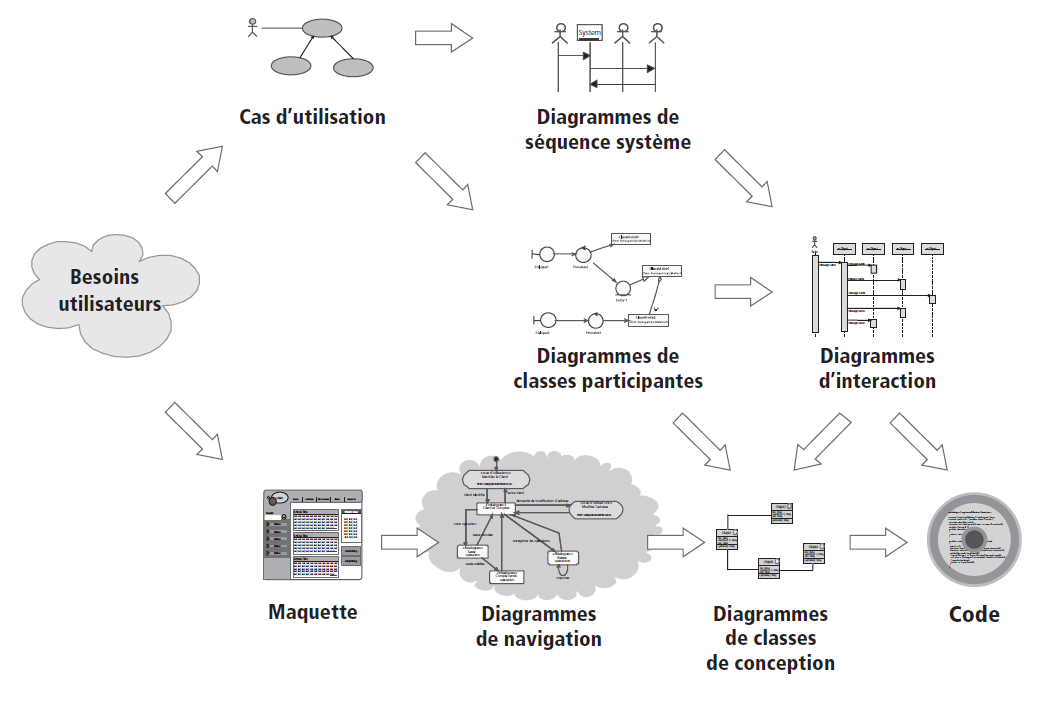
\includegraphics[width=12cm]{images/processus_dev.png}
  \vspace{-10pt}
  \caption{Récapitulatif du processus de développement \cite{5}}
  \label{fig1}
\end{figure}

\vspace{-30pt}
\section{Conclusion}
Ce premier chapitre nous a permis de présenter le cadre général du projet, à
savoir le contexte et la problématique en élaborant une solution à cette
dernière. Nous avons aussi brièvement défini les applications web et les
empreintes digitales. Nous avons conclu par la description du processus de
développement à suivre tout au long du projet.
